\documentclass[conference]{IEEEtran}
\IEEEoverridecommandlockouts

\usepackage{amsmath,amssymb,amsfonts}
\usepackage{graphicx}
\usepackage{booktabs}
\usepackage{array}
\usepackage{algorithm}
\usepackage{algpseudocode}
\usepackage{xcolor}
\usepackage[hidelinks]{hyperref}
\usepackage{url}

\graphicspath{{figures/}}

% --- convenience macros (notation shared with the reference implementation) ---
\newcommand{\Nhat}{\hat{N}}
\newcommand{\Real}{\mathbb{R}}
\newcommand{\cov}{\operatorname{cov}}
\newcommand{\route}{\operatorname{route}}
\newcommand{\Atot}{A_{\mathrm{total}}}

\begin{document}

\title{Four Complementary Estimators of Genetic-Algorithm Population Size
for Relay Placement in Mobile Wireless Sensor Networks, and Their Fusion}

\author{%
\IEEEauthorblockN{SimLab Algorithms Study}
\IEEEauthorblockA{Wireless Sensor Network Optimisation Group\\
\texttt{simlab-algorithms} repository}
}

\maketitle

\begin{abstract}
Choosing the population size of a genetic algorithm (GA) is a classical but
still practically awkward decision: too small and the search loses good
building blocks, too large and it wastes evaluations. We study this decision for
the relay-placement problem in a mobile wireless sensor network (the
\emph{P2} problem), in which a binary chromosome selects a subset of candidate
relay sites so that every mobile sensor remains connected to a sink at all
times. We propose and implement four complementary population-size estimators
that view the problem from different angles: (i) an \emph{inference} estimator
that fits the diminishing returns of converged GA quality against population
size; (ii) an \emph{adjacency} estimator built on the temporal co-occurrence
matrix of the network; (iii) a \emph{routing} estimator built on
shortest-path usage; and (iv) a \emph{MILP-calibrated} estimator that measures
the GA's solution-quality gap relative to a mixed-integer optimum. We then fuse
the four estimates through a conservative envelope, an inverse-variance
weighted average, and a Gaussian Bayesian conjugate update. On a fixed
$64$-candidate, $4$-mobile instance the four methods give
$\Nhat_1{=}22$, $\Nhat_2{=}24$, $\Nhat_3{=}14$ and $\Nhat_4{=}48$; fusion yields
a consensus of $25$ and a conservative recommendation of $48$, while a classical
gambler-ruin bound returns $2839$, two orders of magnitude larger. The methods
agree to within a small constant factor, suggesting that cheap structural and
calibration signals can replace expensive worst-case bounds for practical
population sizing.
\end{abstract}

\begin{IEEEkeywords}
genetic algorithms, population sizing, wireless sensor networks, relay
placement, mixed-integer linear programming, Bayesian fusion.
\end{IEEEkeywords}

\section{Introduction}
\label{sec:intro}
Population size is one of the few GA parameters with a well-developed theory and
yet no convenient practical recipe. The seminal sizing models of Goldberg,
Deb and Clark~\cite{goldberg1992sizing} and the gambler-ruin model of Harik
\emph{et al.}~\cite{harik1999gambler} bound the population needed to avoid losing
a correct building block to genetic drift. These bounds are valuable but
\emph{worst-case}: they scale with $2^{k}$ in the block size $k$ and routinely
recommend populations far larger than what works empirically.

We are motivated by a concrete design task from the \texttt{simlab} toolchain:
multi-objective relay placement for a mobile wireless sensor network
(WSN)~\cite{akyildiz2002survey,younis2008placement}. The decision variable is a
binary chromosome $B\in\{0,1\}^{N}$ over $N$ candidate relay sites, and an
evolutionary algorithm such as NSGA-III~\cite{deb2014nsga3} searches for layouts
that keep mobile sensors connected to a sink while minimising relays. Before
launching such a search, the practitioner must pick a population size.

\paragraph*{Research questions}
(RQ1) Can cheap, instance-specific signals --- search dynamics, network
geometry, routing structure, and exact optima --- each yield a usable
population-size estimate? (RQ2) Do these independent estimates agree, and how
should they be fused into a single recommendation? (RQ3) How do the data-driven
estimates compare with the classical worst-case bound?

\paragraph*{Contributions}
(1) Four complementary, fully-implemented population-size estimators for P2,
each with explicit formulae and diagnostics
(\autoref{sec:m1}--\autoref{sec:m4}). (2) Three fusion strategies --- a
conservative envelope, an inverse-variance weighted average, and a Gaussian
Bayesian conjugate update (\autoref{sec:combined}). (3) An end-to-end,
reproducible evaluation on a fixed P2 instance, contrasting the four estimates
and the classical gambler-ruin bound (\autoref{sec:results}).

\section{Related Work}
\label{sec:related}
\textbf{Population sizing theory.} Holland's schema
theorem~\cite{holland1975adaptation} and Goldberg's building-block
view~\cite{goldberg1989ga,goldberg2002design} frame the GA as a processor of
short, low-order, high-fitness schemata; see~\cite{mitchell1996introduction,
eiben2003introduction} for general treatments. Goldberg, Deb and
Clark~\cite{goldberg1992sizing} sized the population to control decision-making
under fitness noise; Harik \emph{et al.}~\cite{harik1999gambler} recast this as a
one-dimensional gambler-ruin random walk, giving the bound our baseline uses.
Reeves~\cite{reeves1993small} studied very small populations, and
Cant\'u-Paz~\cite{cantupaz2000parallel} and Lobo and
Lima~\cite{harik1999elitist} surveyed adaptive and parallel sizing. Drift
analysis~\cite{he2001drift} relates population and runtime more generally.

\textbf{WSN optimisation with GAs.} Node and relay placement are standard WSN
design problems~\cite{younis2008placement,cheng2008relay}. Multi-objective GAs
are a common solver~\cite{konak2006multiobjective,jourdan2004layout}, with
NSGA-II~\cite{deb2002nsga2} and NSGA-III~\cite{deb2014nsga3} the usual engines.

\textbf{Exact benchmarking.} Mixed-integer linear programming
(MILP)~\cite{wolsey1998integer}, solved by Gurobi~\cite{gurobi2024} or open
solvers such as HiGHS~\cite{huangfu2018highs}, provides optimal or near-optimal
references against which a metaheuristic can be calibrated. Shortest-path
structure is computed with breadth-first search~\cite{cormen2009algorithms}.
Our statistical tooling uses the bootstrap~\cite{efron1993bootstrap} and
Gaussian conjugate updates~\cite{gelman2013bayesian}; firmware-level validation
of layouts uses the COOJA simulator~\cite{osterlind2006cooja}.

\section{Problem Formulation}
\label{sec:problem}
\subsection{The P2 relay-placement problem}
Let $\Omega\subset\Real^2$ be a compact region containing a fixed sink
$s\in\Omega$, a finite set $Q=\{\xi_1,\dots,\xi_N\}$ of candidate relay
positions, and $M$ mobile sensors with trajectories
$\gamma_m:\Real_+\!\to\Omega$. Two devices communicate when within a reach
radius $R$. P2 asks for the smallest subset $P\subseteq Q$ such that, at every
time $t$, every mobile $\gamma_m(t)$ reaches $s$ through a chain of installed,
mutually in-range relays.

\subsection{Chromosome and fitness}
A solution is a binary chromosome $x\in\{0,1\}^{N}$ with $x_j=1$ iff candidate
$j$ is installed. We discretise time into $T$ steps and score $x$ with the
deterministic surrogate fitness used throughout \texttt{simlab}:
\begin{align}
F(x) =\ & w_c\,\mathrm{conn}(x) - w_r\tfrac{\mathrm{relays}(x)}{N}
        - w_h\tfrac{\overline{\mathrm{hops}}(x)}{N} \nonumber\\
       & - w_d\tfrac{\overline{d}(x)}{100} - w_\rho\tfrac{\mathrm{red}(x)}{N},
\label{eq:fitness}
\end{align}
where $\mathrm{conn}(x)\in[0,1]$ is the fraction of (mobile, time) pairs
connected to the sink, $\mathrm{relays}(x)$ the relay count, and the remaining
terms penalise hop count, mean distance and redundancy. Higher $F$ is better.
This is exactly the structural quantity the MILP minimises, so GA and MILP
solutions are directly comparable.

\subsection{The population-sizing problem}
Given P2 and a confidence level $1-\alpha$, find the smallest population size
$\Nhat$ such that a GA with population $\Nhat$ returns a good solution with
probability at least $1-\alpha$. We attack this through four estimators and a
fusion step.

\section{Method 1: Inference via Inter-Sample Differences}
\label{sec:m1}
\subsection{Diminishing returns of converged quality}
Run the GA at a ladder of population sizes $n$ and record the converged best
fitness $F^*(n)$, averaged over seeds. Each extra individual contributes
marginal information with diminishing returns, which we model as the saturating
growth
\begin{equation}
F^*(n) = F_\infty - A\,e^{-n/\tau}, \qquad A>0,\ \tau>0.
\label{eq:m1-model}
\end{equation}
The remaining improvement beyond $n$ is $\rho(n)=F_\infty-F^*(n)=A\,e^{-n/\tau}$,
and the marginal gain of one individual is
\begin{equation}
\frac{dF^*}{dn} = \frac{A}{\tau}\,e^{-n/\tau}.
\label{eq:m1-marginal}
\end{equation}
Declaring the population large enough once the \emph{relative} remaining
improvement drops below a tolerance $\varepsilon$ gives
$e^{-n/\tau}\le\varepsilon$, hence the estimator
\begin{equation}
\boxed{\;\Nhat_1 = \left\lceil \tau\,\ln\!\frac{1}{\varepsilon}\right\rceil.\;}
\label{eq:m1-est}
\end{equation}
\autoref{eq:m1-est} is scale-free in the units of $F$ and captures
$(1-\varepsilon)$ of the quality an unbounded population could reach. A
$95\%$ confidence interval follows from a bootstrap over GA
seeds~\cite{efron1993bootstrap}: resample seeds, recompute the per-$n$ means,
refit~\eqref{eq:m1-model}, recompute~\eqref{eq:m1-est}.

\begin{algorithm}[!t]
\caption{Method 1 estimate}
\label{alg:m1}
\begin{algorithmic}[1]
\Require population sizes $\{n_k\}$, seeds $\{s\}$, tolerance $\varepsilon$
\For{each $n_k$, each seed $s$} run GA; record $F^*_{k,s}$ \EndFor
\State $\bar F_k \gets \mathrm{mean}_s F^*_{k,s}$
\State $(F_\infty, A, \tau) \gets \textsc{FitSat}(\{(n_k,\bar F_k)\})$
  \Comment{$\tau$-grid + linear least squares}
\State $\Nhat_1 \gets \lceil \tau\ln(1/\varepsilon)\rceil$
\State $\mathrm{CI} \gets$ bootstrap over seeds
\State \Return $\Nhat_1$, CI
\end{algorithmic}
\end{algorithm}

\subsection{Inter-sample information gain (corroboration)}
From one large reference run we take the ordered stream of distinct evaluated
individuals $x_1,x_2,\dots$ and form the ``difference vectors'' the search
produces: the inter-sample Hamming distance $h_j=\lVert x_j\oplus x_{j-1}\rVert_1$,
large while exploring and shrinking on convergence, and the cumulative best
$B(j)=\max_{i\le j}F(x_i)$. Fitting~\eqref{eq:m1-model} to $B(j)$ gives an
information scale $\tau_{\mathrm{info}}$ and a sampling budget
$j_{95}=\tau_{\mathrm{info}}\ln(1/\varepsilon)$ that corroborates the
population-scale saturation.

\subsection{Complexity}
Building the curve costs the GA sweep,
$O(|\text{sizes}|\cdot|\text{seeds}|\cdot P\cdot G\cdot C_{\mathrm{eval}})$; the
fit is an $O(n_\tau\cdot K)$ grid search with a closed-form linear solve per grid
point.

\autoref{fig:m1-sat} shows the saturation curve and $\Nhat_1$;
\autoref{fig:m1-marg} the marginal gain and confidence band;
\autoref{fig:m1-info} the inter-sample information-gain view.

\begin{figure}[!t]
\centering
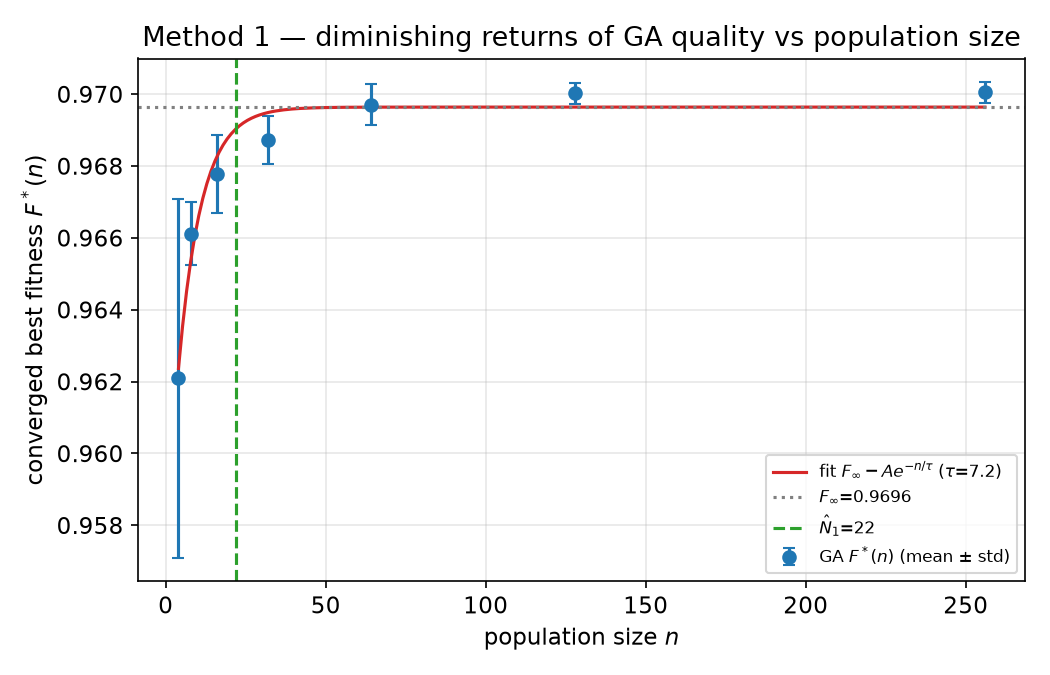
\includegraphics[width=\columnwidth]{m1_saturation.png}
\caption{Method 1: converged GA fitness $F^*(n)$ versus population size with the
fitted saturating model~\eqref{eq:m1-model} and $\Nhat_1$.}
\label{fig:m1-sat}
\end{figure}

\begin{figure}[!t]
\centering
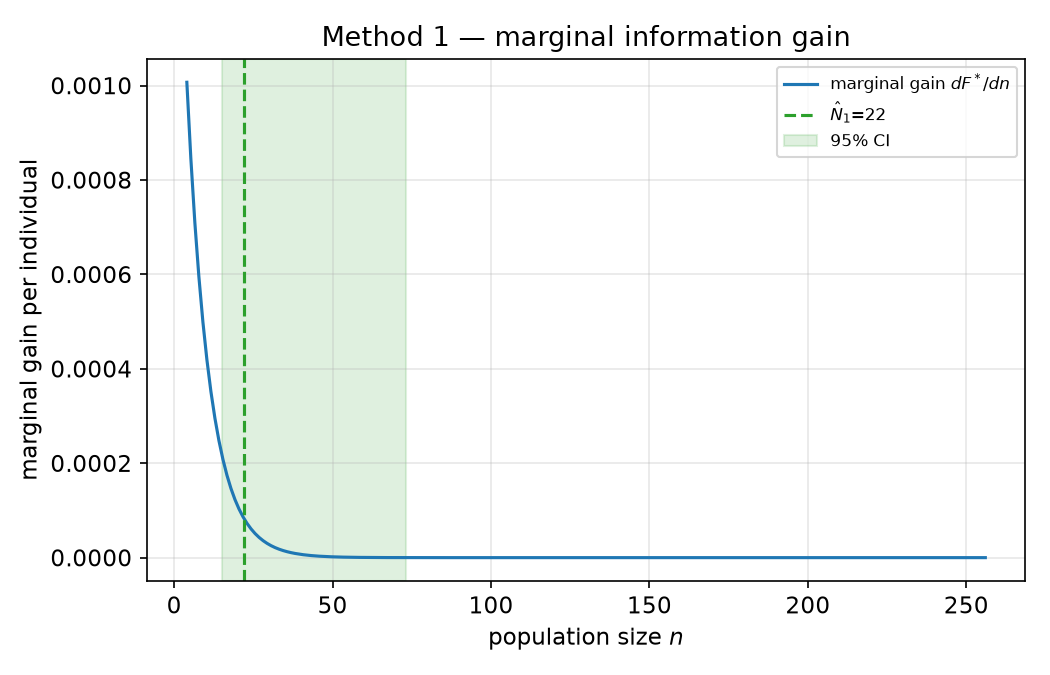
\includegraphics[width=\columnwidth]{m1_marginal.png}
\caption{Method 1: marginal information gain per
individual~\eqref{eq:m1-marginal}; the dashed line marks $\Nhat_1$ and the band
its $95\%$ bootstrap CI.}
\label{fig:m1-marg}
\end{figure}

\begin{figure}[!t]
\centering
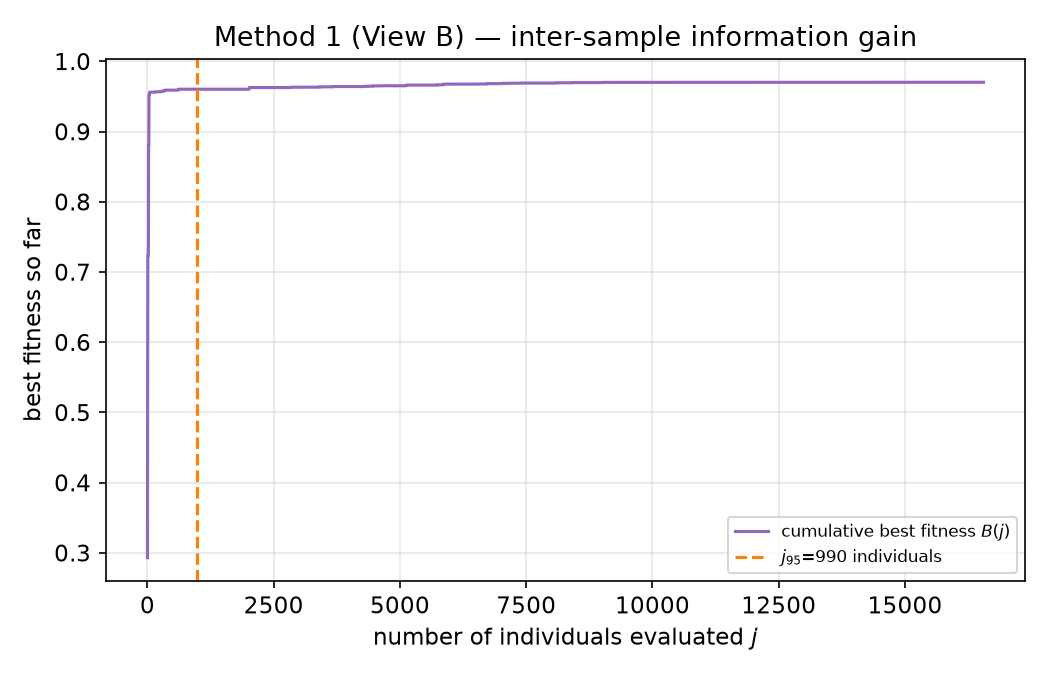
\includegraphics[width=\columnwidth]{m1_infogain.png}
\caption{Method 1 (corroboration): cumulative best fitness $B(j)$ versus the
number of individuals evaluated, with the sampling budget $j_{95}$.}
\label{fig:m1-info}
\end{figure}

\section{Method 2: Adjacency-Matrix Temporal Dynamics}
\label{sec:m2}
With the canonical layout $K=1+N+M=[\text{sink},\text{candidates},\text{mobiles}]$,
the per-timestep adjacency encodes geometric reachability,
\begin{equation}
A(t)[u,v]=1 \iff u\neq v \ \wedge\ \lVert p_u(t)-p_v(t)\rVert\le R,
\label{eq:m2-adj}
\end{equation}
and the accumulated co-occurrence matrix is
$\Atot[u,v]=\sum_{t=1}^{T}A(t)[u,v]\in[0,T]$ (\autoref{fig:m2-heat}). The
mobile-coverage score of a candidate $u$ is
\begin{equation}
\cov(u)=\sum_{m\in\text{mobiles}}\Atot[u,m]\in[0,TM],
\label{eq:m2-cov}
\end{equation}
shown sorted in \autoref{fig:m2-cov} and spatially in \autoref{fig:m2-spatial}.
The indispensable candidates at coverage fraction $\theta$ are
$C_\theta=\#\{u\in Q:\cov(u)\ge\theta\,TM\}$.

\paragraph*{Temporal convergence}
Using partial coverage $\cov_t(u)=\sum_{\tau\le t}\sum_m A(\tau)[u,m]$, the
indispensable count $|C_\theta(t)|$ is non-decreasing and saturates once the last
indispensable candidate has accumulated enough coverage; we report the first
$t^*$ at which it reaches its final value (\autoref{fig:m2-conv}).

\paragraph*{Estimator}
The minimum number of relays covering the whole trajectory is lower-bounded by
$C_\theta$; spreading those indispensable genes across blocks of mean size
$\bar k=N/B$ means a random individual carries all of them with low probability,
giving
\begin{equation}
\boxed{\;\Nhat_2=\left\lceil C_\theta\,(1/\alpha)^{1/\bar k}\right\rceil.\;}
\label{eq:m2-est}
\end{equation}
The factor $(1/\alpha)^{1/\bar k}$ is the per-critical-region multiplier needed
so the probability of missing a required gene falls to $\alpha$. We sweep
$\theta\in[0.05,0.20]$ for an uncertainty interval.

\begin{figure}[!t]
\centering
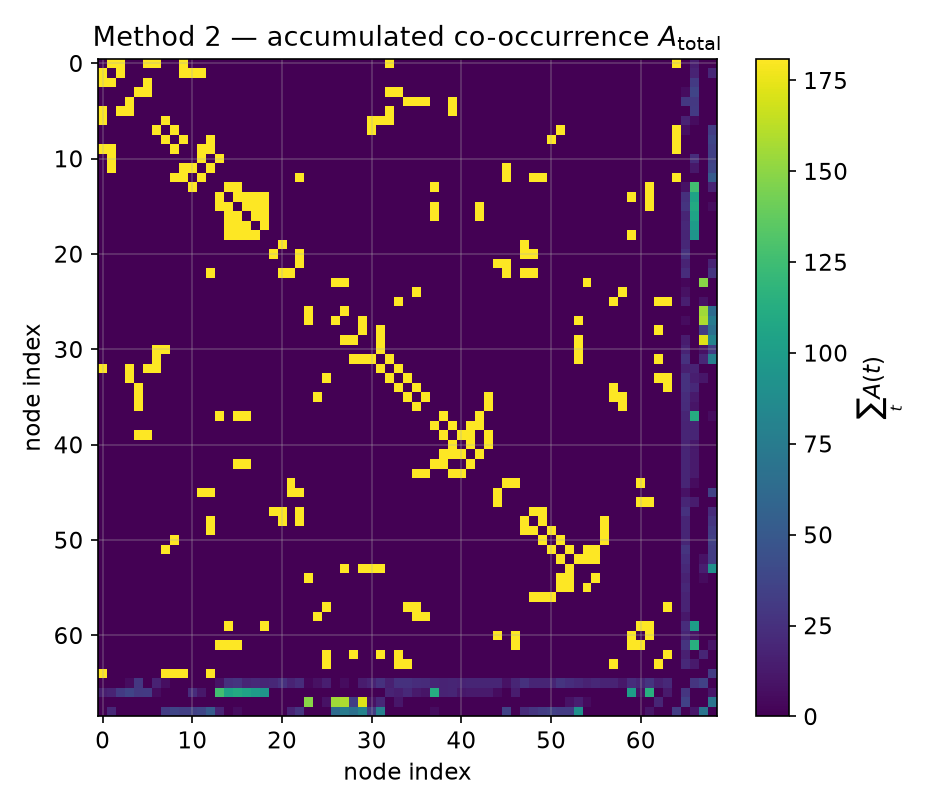
\includegraphics[width=0.86\columnwidth]{m2_heatmap.png}
\caption{Method 2: accumulated co-occurrence matrix $\Atot$~\eqref{eq:m2-adj}.}
\label{fig:m2-heat}
\end{figure}

\begin{figure}[!t]
\centering
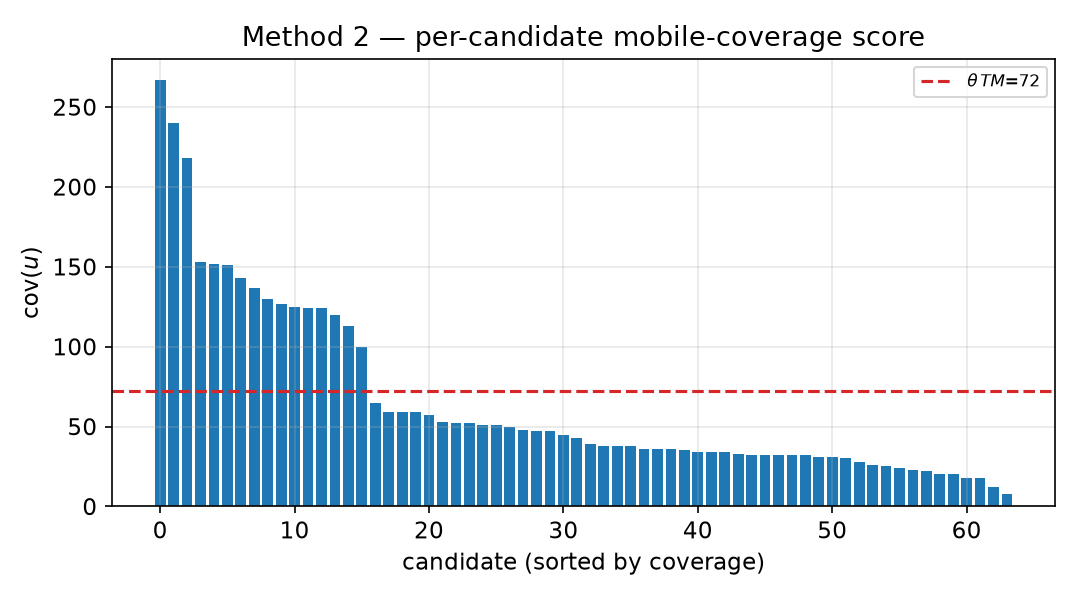
\includegraphics[width=\columnwidth]{m2_coverage.png}
\caption{Method 2: per-candidate coverage $\cov(u)$~\eqref{eq:m2-cov}, sorted;
the dashed line is the indispensability threshold $\theta\,TM$.}
\label{fig:m2-cov}
\end{figure}

\begin{figure}[!t]
\centering
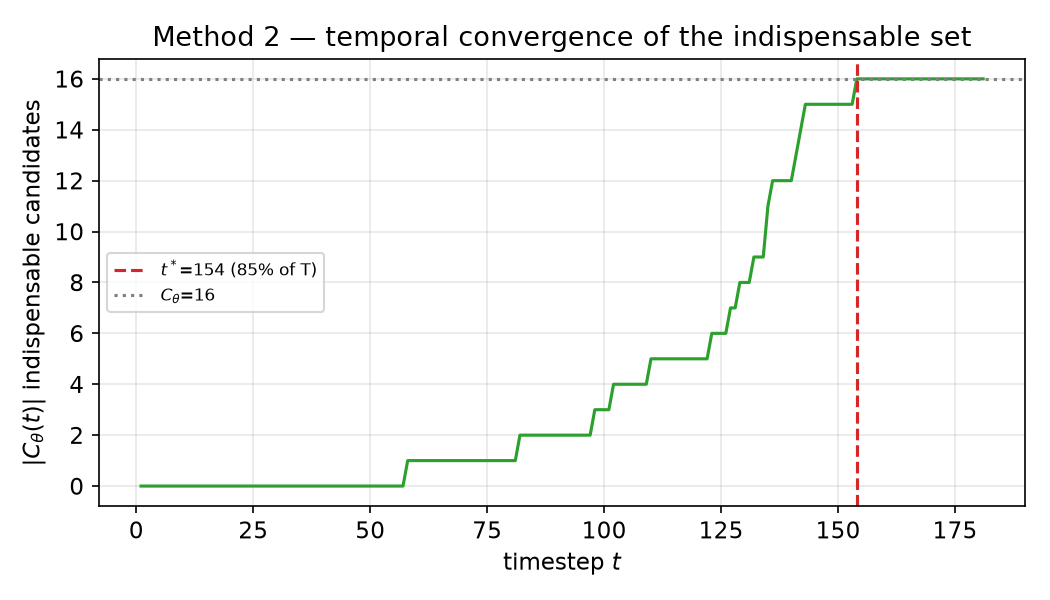
\includegraphics[width=\columnwidth]{m2_convergence.png}
\caption{Method 2: temporal convergence of the indispensable set
$|C_\theta(t)|$.}
\label{fig:m2-conv}
\end{figure}

\begin{figure}[!t]
\centering
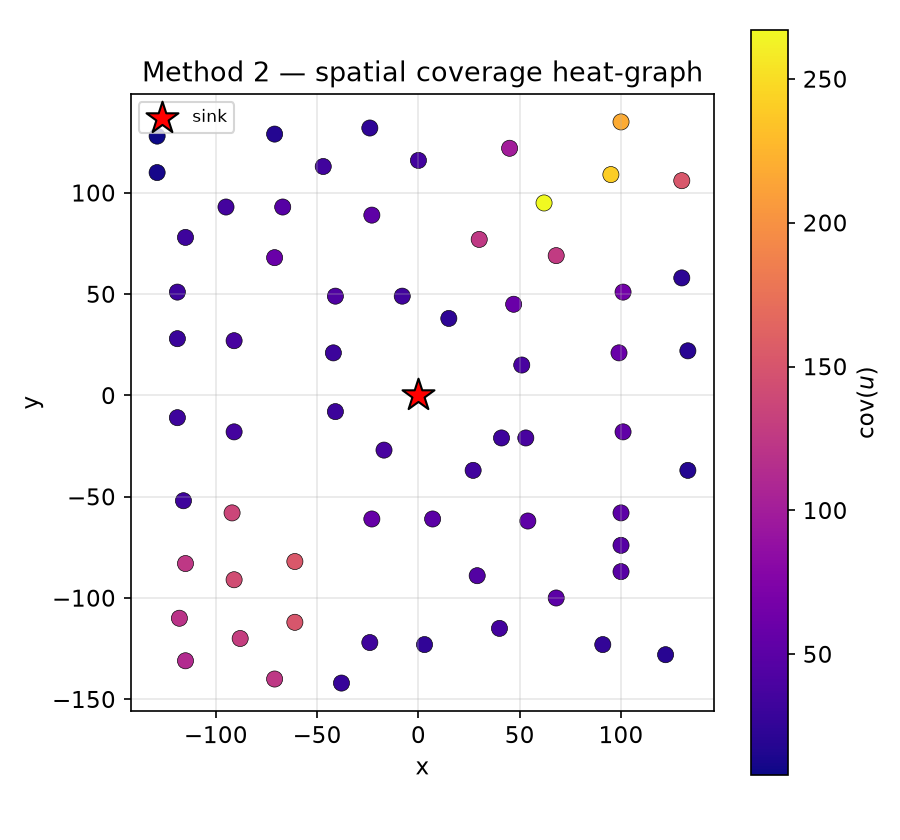
\includegraphics[width=0.82\columnwidth]{m2_spatial.png}
\caption{Method 2: candidates coloured by coverage $\cov(u)$; the star is the
sink.}
\label{fig:m2-spatial}
\end{figure}

\section{Method 3: Routing-Matrix Variant}
\label{sec:m3}
Method 3 mirrors Method 2 but replaces \emph{reachability} with \emph{usage}.
At each $t$ we run one breadth-first search from the
sink~\cite{cormen2009algorithms} in $A(t)$ and keep only nodes and edges on a
chosen shortest mobile-to-sink path, forming the routing matrix $R(t)$. With
$\text{node\_acc}[u]=\sum_t \#\{\text{mobiles whose shortest path uses }u\}$,
the routing score is
\begin{equation}
\route(u)=\frac{\text{node\_acc}[u]}{TM}\in[0,1],
\label{eq:m3-route}
\end{equation}
and the critical relays are $R_\phi=\#\{u\in Q:\route(u)\ge\phi\}$. The estimator
is analogous to~\eqref{eq:m2-est}:
\begin{equation}
\boxed{\;\Nhat_3=\left\lceil |R_\phi|\,(1/\alpha)^{1/\bar k}\right\rceil.\;}
\label{eq:m3-est}
\end{equation}

\subsection{$A(t)$ versus $R(t)$: what each captures}
$A(t)$ is symmetric reachability --- it counts every in-range pair whether or not
traffic uses it, so it \emph{over-counts}. $R(t)$ is directed usage --- a
candidate scores only when it is an actual relay hop, so $R(t)\subseteq A(t)$ and
$\route(u)$ is sparser than $\cov(u)$. The gap between them is diagnostic: a high
$\cov$ with low $\route$ marks \emph{redundant} coverage, whereas a moderate
$\cov$ with high $\route$ marks a \emph{routing bottleneck}. Empirically (see
\autoref{sec:results}) only $9$ candidates are routing-critical against $16$
coverage-indispensable, so $\Nhat_3<\Nhat_2$. Figures
\ref{fig:m3-edge}--\ref{fig:m3-spatial} report the edge-usage heatmap, the sorted
routing scores, the temporal convergence of $|R_\phi(t)|$, and the spatial
routing map.

\begin{figure}[!t]
\centering
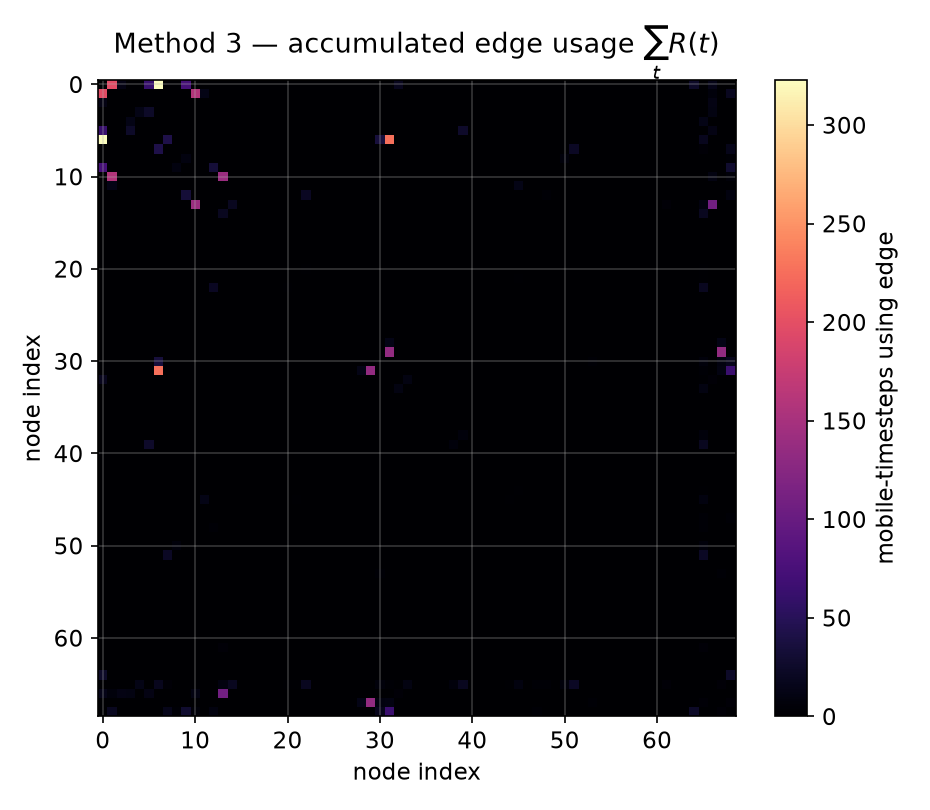
\includegraphics[width=0.86\columnwidth]{m3_edge_heatmap.png}
\caption{Method 3: accumulated edge usage $\sum_t R(t)$.}
\label{fig:m3-edge}
\end{figure}

\begin{figure}[!t]
\centering
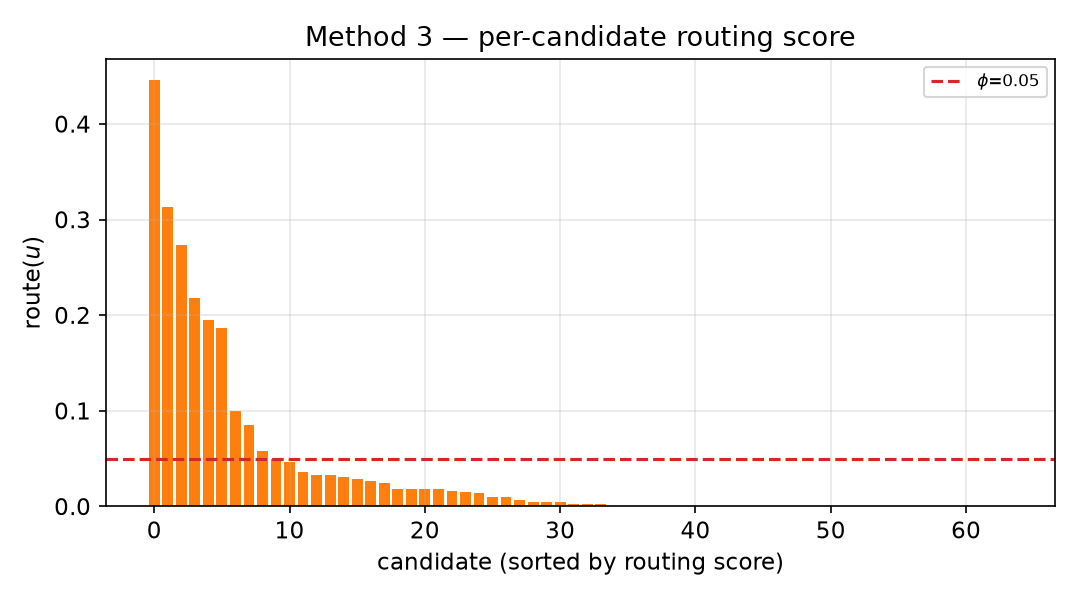
\includegraphics[width=\columnwidth]{m3_route.png}
\caption{Method 3: per-candidate routing score $\route(u)$~\eqref{eq:m3-route},
sorted; the dashed line is the criticality threshold $\phi$.}
\label{fig:m3-route}
\end{figure}

\begin{figure}[!t]
\centering
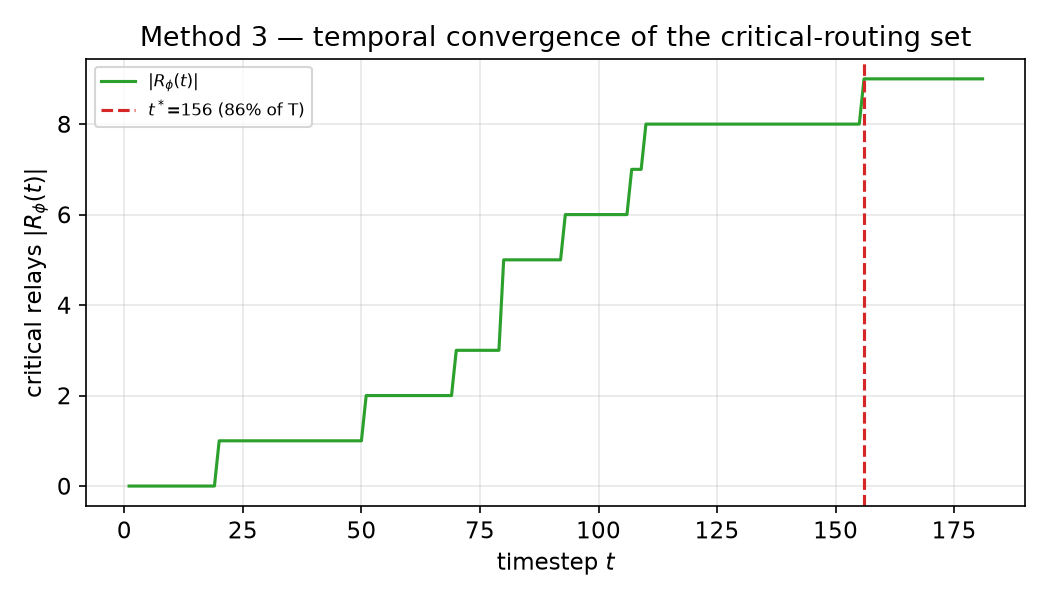
\includegraphics[width=\columnwidth]{m3_convergence.png}
\caption{Method 3: temporal convergence of the critical-routing set
$|R_\phi(t)|$.}
\label{fig:m3-conv}
\end{figure}

\begin{figure}[!t]
\centering
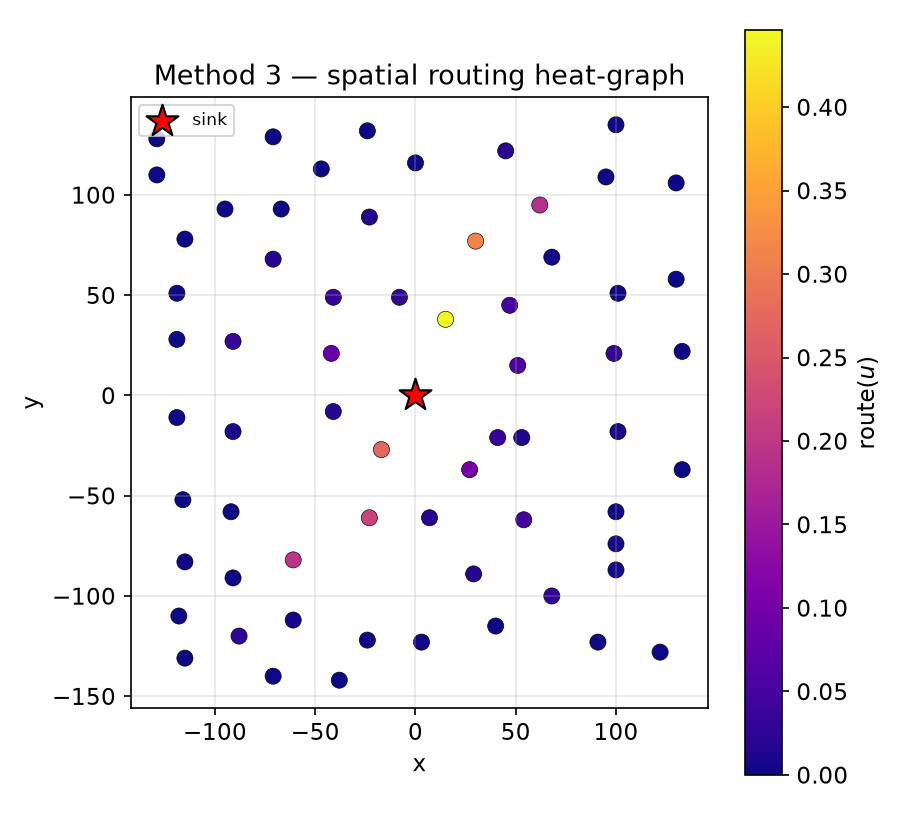
\includegraphics[width=0.82\columnwidth]{m3_spatial.png}
\caption{Method 3: candidates coloured by routing score $\route(u)$.}
\label{fig:m3-spatial}
\end{figure}

\section{Method 4: MILP-Based Calibration}
\label{sec:m4}
A MILP sweep solves the same instance to (near-)optimality, giving a
ground-truth reference. P2 quality is the relay count at full connectivity, so
the reference optimum is
\begin{equation}
r_{\mathrm{opt}}=\min\{\,\mathrm{relays}(x): x\ \text{optimal MILP solve}\,\}.
\label{eq:m4-ropt}
\end{equation}
For population $n$, with $r_{\mathrm{GA}}(n)$ the GA's converged relay count at
full connectivity (seed-averaged), the optimality gap is
\begin{equation}
\mathrm{gap}(n)=\frac{r_{\mathrm{GA}}(n)-r_{\mathrm{opt}}}{r_{\mathrm{opt}}}\ge 0,
\label{eq:m4-gap}
\end{equation}
which we calibrate with a decaying curve
$\mathrm{gap}(n)=g_\infty+G\,e^{-n/\tau}$. Inverting at a target tolerance
$\tau_{\mathrm{gap}}$ gives
\begin{equation}
\boxed{\;\Nhat_4=\left\lceil \tau\,\ln\!\frac{G}{\tau_{\mathrm{gap}}-g_\infty}
\right\rceil,\quad \tau_{\mathrm{gap}}>g_\infty.\;}
\label{eq:m4-est}
\end{equation}
If $\tau_{\mathrm{gap}}\le g_\infty$ the target lies below the achievable floor.
\autoref{fig:m4-gap} shows the calibrated gap and $\Nhat_4$;
\autoref{fig:m4-land} scores the MILP solutions with the surrogate and marks
$r_{\mathrm{opt}}$.

\begin{figure}[!t]
\centering
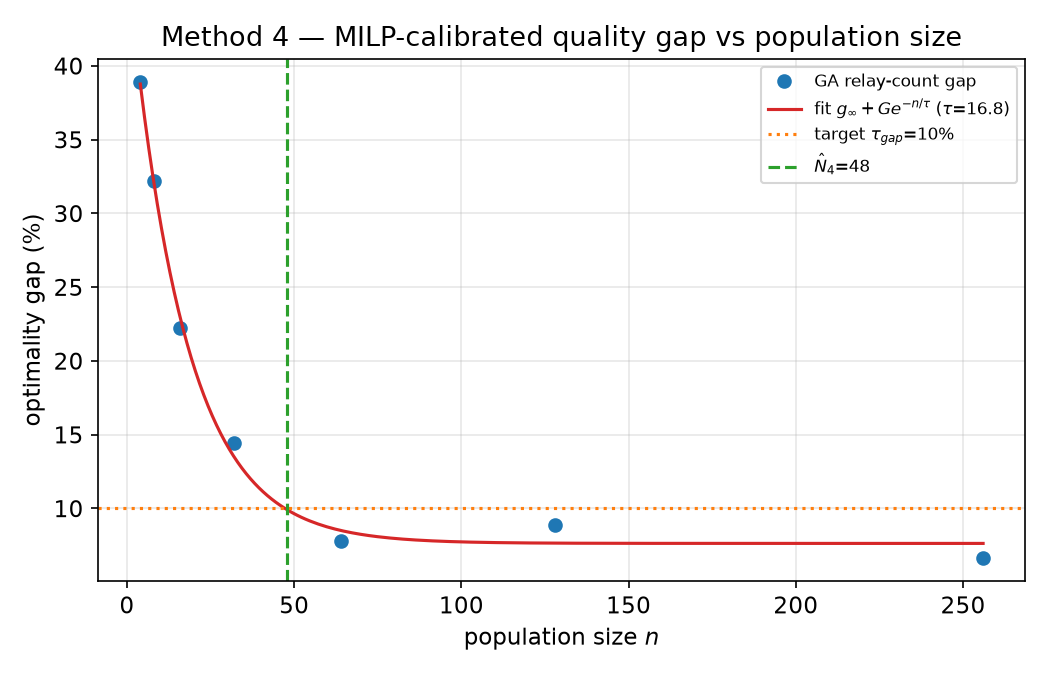
\includegraphics[width=\columnwidth]{m4_gap.png}
\caption{Method 4: GA optimality gap~\eqref{eq:m4-gap} versus population size,
the calibration fit, the target $\tau_{\mathrm{gap}}$ and $\Nhat_4$.}
\label{fig:m4-gap}
\end{figure}

\begin{figure}[!t]
\centering
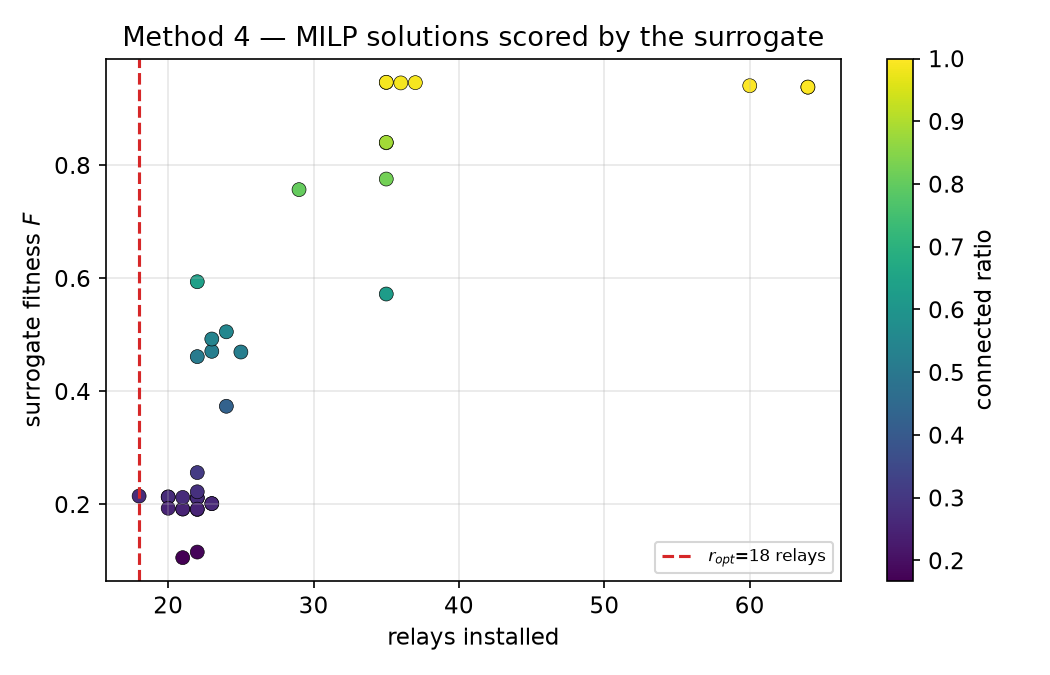
\includegraphics[width=\columnwidth]{m4_landscape.png}
\caption{Method 4: MILP solutions scored by the surrogate (relays vs.\ fitness,
coloured by connectivity); the dashed line is $r_{\mathrm{opt}}$.}
\label{fig:m4-land}
\end{figure}

\section{Combined Estimator}
\label{sec:combined}
Each method returns $(\Nhat_i,\sigma_i)$. We fuse them three ways.

\paragraph*{Conservative envelope}
$\;\Nhat_{\mathrm{env}}=\max_i \Nhat_i$, guaranteeing every criterion is met.

\paragraph*{Inverse-variance weighted average}
With precisions $w_i=1/\sigma_i^2$,
\begin{equation}
\Nhat_{\mathrm{wavg}}=\frac{\sum_i w_i \Nhat_i}{\sum_i w_i},\qquad
\mathrm{Var}=\frac{1}{\sum_i w_i}.
\label{eq:wavg}
\end{equation}

\paragraph*{Bayesian Gaussian fusion}
Treating $\Nhat_i\sim\mathcal{N}(N^*,\sigma_i^2)$ with a weakly-informative prior
$N^*\sim\mathcal{N}(\mu_0,\sigma_0^2)$~\cite{gelman2013bayesian}, the posterior is
Gaussian with
\begin{align}
\frac{1}{\sigma_{\mathrm{post}}^2} &= \frac{1}{\sigma_0^2}+\sum_i\frac{1}{\sigma_i^2},
\label{eq:bayes-prec}\\
\mu_{\mathrm{post}} &= \sigma_{\mathrm{post}}^2\!\left(\frac{\mu_0}{\sigma_0^2}
   +\sum_i\frac{\Nhat_i}{\sigma_i^2}\right),
\label{eq:bayes-mean}
\end{align}
and a $95\%$ credible interval $\mu_{\mathrm{post}}\pm1.96\,\sigma_{\mathrm{post}}$.

\paragraph*{Gaussian vs.\ Poisson}
A Poisson model would force $\mathrm{Var}=\mathrm{mean}$. The four estimates are
strongly over-dispersed (dispersion ratio $\approx 8$, \autoref{sec:results}),
violating that assumption, so the Gaussian model is selected.

\section{Experimental Setup}
\label{sec:setup}
\textbf{Instance.} A single fixed P2 instance (\texttt{ind2}): $N=64$ candidate
sites, $M=4$ mobile sensors on closed/round-trip trajectories, reach radius
$R=50$, region $[-150,150]^2$, sink at the origin, horizon $T=181$ steps.

\textbf{GA.} Binary chromosome of length $N$; uniform crossover ($p_c=0.9$),
bit-flip mutation ($p_m=1/N$), $3$-tournament selection, elitism $1$,
Bernoulli$(0.5)$ initialisation, $80$ generations. Population sizes
$n\in\{4,8,16,32,64,128,256\}$, each over seeds $\{0,1,2,3,4\}$. Fitness is the
deterministic surrogate~\eqref{eq:fitness} with default weights
$(w_c,w_r,w_h,w_d,w_\rho)=(1,0.05,0.05,0.05,0.02)$.

\textbf{MILP.} The mobile-coverage MILP from the \texttt{p2-milp-sweep}
experiment, solved with HiGHS~\cite{huangfu2018highs}; $36$ optimal solves over a
$(C_0,k_{\mathrm{decay}},B)$ grid provide the reference set.

\textbf{Settings.} $\alpha=0.05$; Method 1 $\varepsilon=0.05$; Method 2/3 mean
block size $\bar k = N/8 = 8$; Method 4 target gap $\tau_{\mathrm{gap}}=0.10$.
Confidence intervals use $1000$ bootstrap resamples. All code runs on a single
Python interpreter (NumPy, Matplotlib); no GPU.

\section{Results and Discussion}
\label{sec:results}
\subsection{Per-method estimates}
\textbf{Method 1.} The converged-fitness curve fits~\eqref{eq:m1-model} tightly
($F_\infty=0.970$, $A=0.013$, $\tau=7.2$, residual sum of squares
$1.6\times10^{-6}$), giving $\Nhat_1=22$ with $95\%$ CI $[15,73]$
(\autoref{fig:m1-sat},\,\autoref{fig:m1-marg}). The inter-sample view
(\autoref{fig:m1-info}) saturates after $\approx 990$ individuals, with a mean
inter-sample Hamming distance of $29.5/64$, confirming broad exploration before
convergence.

\textbf{Method 2.} At $\theta=0.10$ there are $C_\theta=16$ indispensable
candidates, yielding $\Nhat_2=24$. The indispensable set is only fully revealed
late in the trajectory ($t^*=154/181$, $85\%$), confirming that the mobile tour
exercises distinct regions over time (\autoref{fig:m2-conv}).

\textbf{Method 3.} Only $|R_\phi|=9$ candidates are routing-critical at
$\phi=0.05$, giving $\Nhat_3=14$. The routing view is strictly sparser than the
coverage view --- the expected consequence of $R(t)\subseteq A(t)$ --- and the
network stays fully connected at all timesteps under the full candidate set.

\textbf{Method 4.} The MILP reference optimum is $r_{\mathrm{opt}}=18$ relays.
The GA gap falls from $39\%$ at $n=4$ to $7\%$ at $n=256$, fitting
$g_\infty=0.076$, $G=0.40$, $\tau=16.8$; reaching the $10\%$ target needs
$\Nhat_4=48$ with $95\%$ CI $[32,72]$ (\autoref{fig:m4-gap}). Notably the GA's
best layout also uses $18$ relays, matching the MILP optimum and validating both
solvers (\autoref{fig:m4-land}).

\subsection{Fusion}
\autoref{tab:summary} collects all estimates. The four methods span $14$--$48$,
i.e.\ within a factor of $\approx 3.4$, despite using entirely different signals.
Inverse-variance weighting~\eqref{eq:wavg} places most weight on Method 3
($w_3=0.49$, smallest $\sigma$) and gives $\Nhat_{\mathrm{wavg}}=25$; the Bayesian
posterior~\eqref{eq:bayes-mean} agrees at $25$ with credible interval $[14,35]$.
The conservative envelope is $48$, driven by Method 4. The empirical dispersion
ratio is $\approx 8$, confirming the Gaussian (not Poisson) choice.

\begin{table}[!t]
\centering
\caption{Population-size estimates and fusion on the \texttt{ind2} instance.}
\label{tab:summary}
\small
\begin{tabular}{lrrrrr}
\toprule
Estimator & $\hat N$ & raw & CI low & CI high & $\sigma$ \\
\midrule
M1 inference (diminishing returns) & 22 & 21.64 & 15.1 & 73.1 & 14.8 \\
M2 adjacency coverage & 24 & 23.27 & 9.0 & 53.0 & 14.55 \\
M3 routing criticality & 14 & 13.09 & 6.0 & 27.0 & 7.47 \\
M4 MILP calibration & 48 & 47.27 & 32.0 & 71.8 & 10.17 \\
\midrule
COMBINED conservative envelope & 48 & -- & -- & -- & -- \\
\midrule
COMBINED weighted average & 25 & 24.41 & 14.2 & 34.6 & 5.21 \\
\midrule
COMBINED Bayesian fusion & 25 & 24.44 & 14.3 & 34.6 & 5.17 \\
\bottomrule
\end{tabular}
\end{table}

\begin{figure}[!t]
\centering
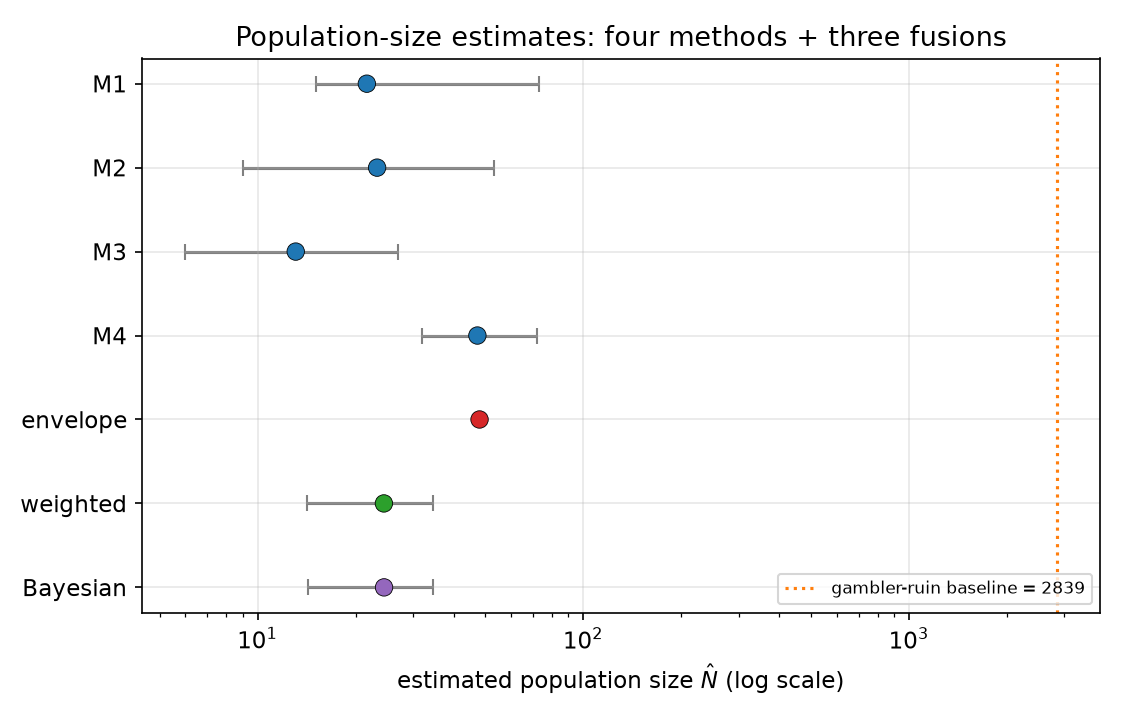
\includegraphics[width=\columnwidth]{combined.png}
\caption{All four estimates (with uncertainty) and the three fusions, on a log
axis; the dotted line is the gambler-ruin baseline ($2839$).}
\label{fig:combined}
\end{figure}

\subsection{Comparison with the classical bound}
The gambler-ruin bound~\cite{harik1999gambler} on the same instance returns
$2839$ --- about two orders of magnitude above the data-driven estimates
(\autoref{fig:combined}). This is consistent with its worst-case nature: the
$2^{\bar k-1}$ factor dominates for $\bar k=8$. For practical sizing, the
calibrated and structural estimates ($14$--$48$) are far more actionable, while
the bound remains a safe but loose ceiling.

\subsection{Threats to validity}
Results are on a single instance, so the absolute numbers should be read as a
proof of concept rather than a universal recommendation; the cross-method
agreement is the transferable finding. The surrogate fitness, while structurally
faithful and consistent between GA and MILP, is not a packet-level simulation;
COOJA validation~\cite{osterlind2006cooja} is left to future work. Methods 2 and
3 use a heuristic threshold ($\theta$, $\phi$) whose sweep we report as the
interval.

\section{Conclusion}
\label{sec:conclusion}
We presented four complementary, fully-reproducible estimators of GA population
size for mobile-WSN relay placement, and three ways to fuse them. On a fixed
instance they agree within a small factor ($\Nhat\in[14,48]$), recommend a
consensus of $25$ and a conservative $48$, and expose the classical gambler-ruin
bound ($2839$) as needlessly large for practical use. The estimators are cheap:
Methods 2 and 3 are pure geometry/graph computations, and Method 4 reuses an
existing MILP sweep. Future work will (i) repeat the study across a library of
instances to learn transferable fusion weights, (ii) validate the chosen
populations against NSGA-III runs and COOJA, and (iii) develop the per-block
meta-estimator that combines coverage and routing criticality at the block
level.

\section*{Reproducibility}
All code, data and figures are in the \texttt{simlab-algorithms} repository:
\texttt{ga/} (GA engine and runs), \texttt{methods/} (the four estimators and the
fusion), and \texttt{results/} (raw outputs and the figures used here).
\texttt{run\_all.sh} regenerates every result and this paper.

\bibliographystyle{IEEEtran}
\bibliography{references}

\end{document}
